
\subsection{Principio de funcionamiento de Amperímetro}
Un amperímetro de bobina móvil se construye utilizando un galvanómetro, un dispositivo muy sensible a pequeñas magnitudes de corriente. El principio básico de este amperímetro es medir la corriente eléctrica que fluye a través de un circuito; sin embargo, dado que el galvanómetro está diseñado para medir corrientes muy bajas, es necesario adaptarlo para poder medir rangos más grandes de corriente sin dañar el dispositivo.

Para lograr esto, se utiliza un divisor de corriente mediante una resistencia shunt en paralelo con el galvanómetro. Esta resistencia, que generalmente tiene un valor muy bajo comparada a la resistencia interna del galvanómetro, permite que una porción de la corriente fluya a través de ella, protegiendo el galvanómetro. De este modo, solo una fracción de la corriente total pasa por el galvanómetro, permitiendo que se utilice para medir corrientes mucho mayores sin que el dispositivo se dañe.

\subsubsection{Cálculo de Resistencias Shunt}
La resistencia shunt $R_s$ se calcula teniendo en cuenta la corriente máxima que se desea medir y la resistencia $R_g$ interna del galvanómetro. El objetivo es asegurar que cuando se mida la corriente máxima, la corriente que pase por el galvanómetro no exceda su corriente máxima admisible $I_{g\ max}$, la cual es determinada por la sensibilidad $s$ del galvanómetro como $I_{g\ max} = 1/s$.

Una vez fijada la corriente máxima para el galvanómetro, la resistencia shunt necesaria para cada rango se determina a partir de la siguiente fórmula:

\begin{equation}
    R_{sh} = R_g \cdot \frac{I_m}{I_{\text{rango}} - I_m}
    \label{eq:Rsh}
\end{equation}

Donde $I_{rango}$ es la corriente máxima que se desea medir en un rango específico del amperímetro.

\subsubsection{Fijación de Resistencia de Calibración}
La resistencia de calibración es una resistencia adicional que se coloca en paralelo con el galvanómetro, y se debe ajustar para asegurar que la corriente que pasa por el galvanómetro sea precisamente la corriente máxima que puede soportar para cuando se está midiendo la corriente de rango cuando y que se alcance la máxima deflexión de la aguja.


\begin{figure}[h!]
  \centering
  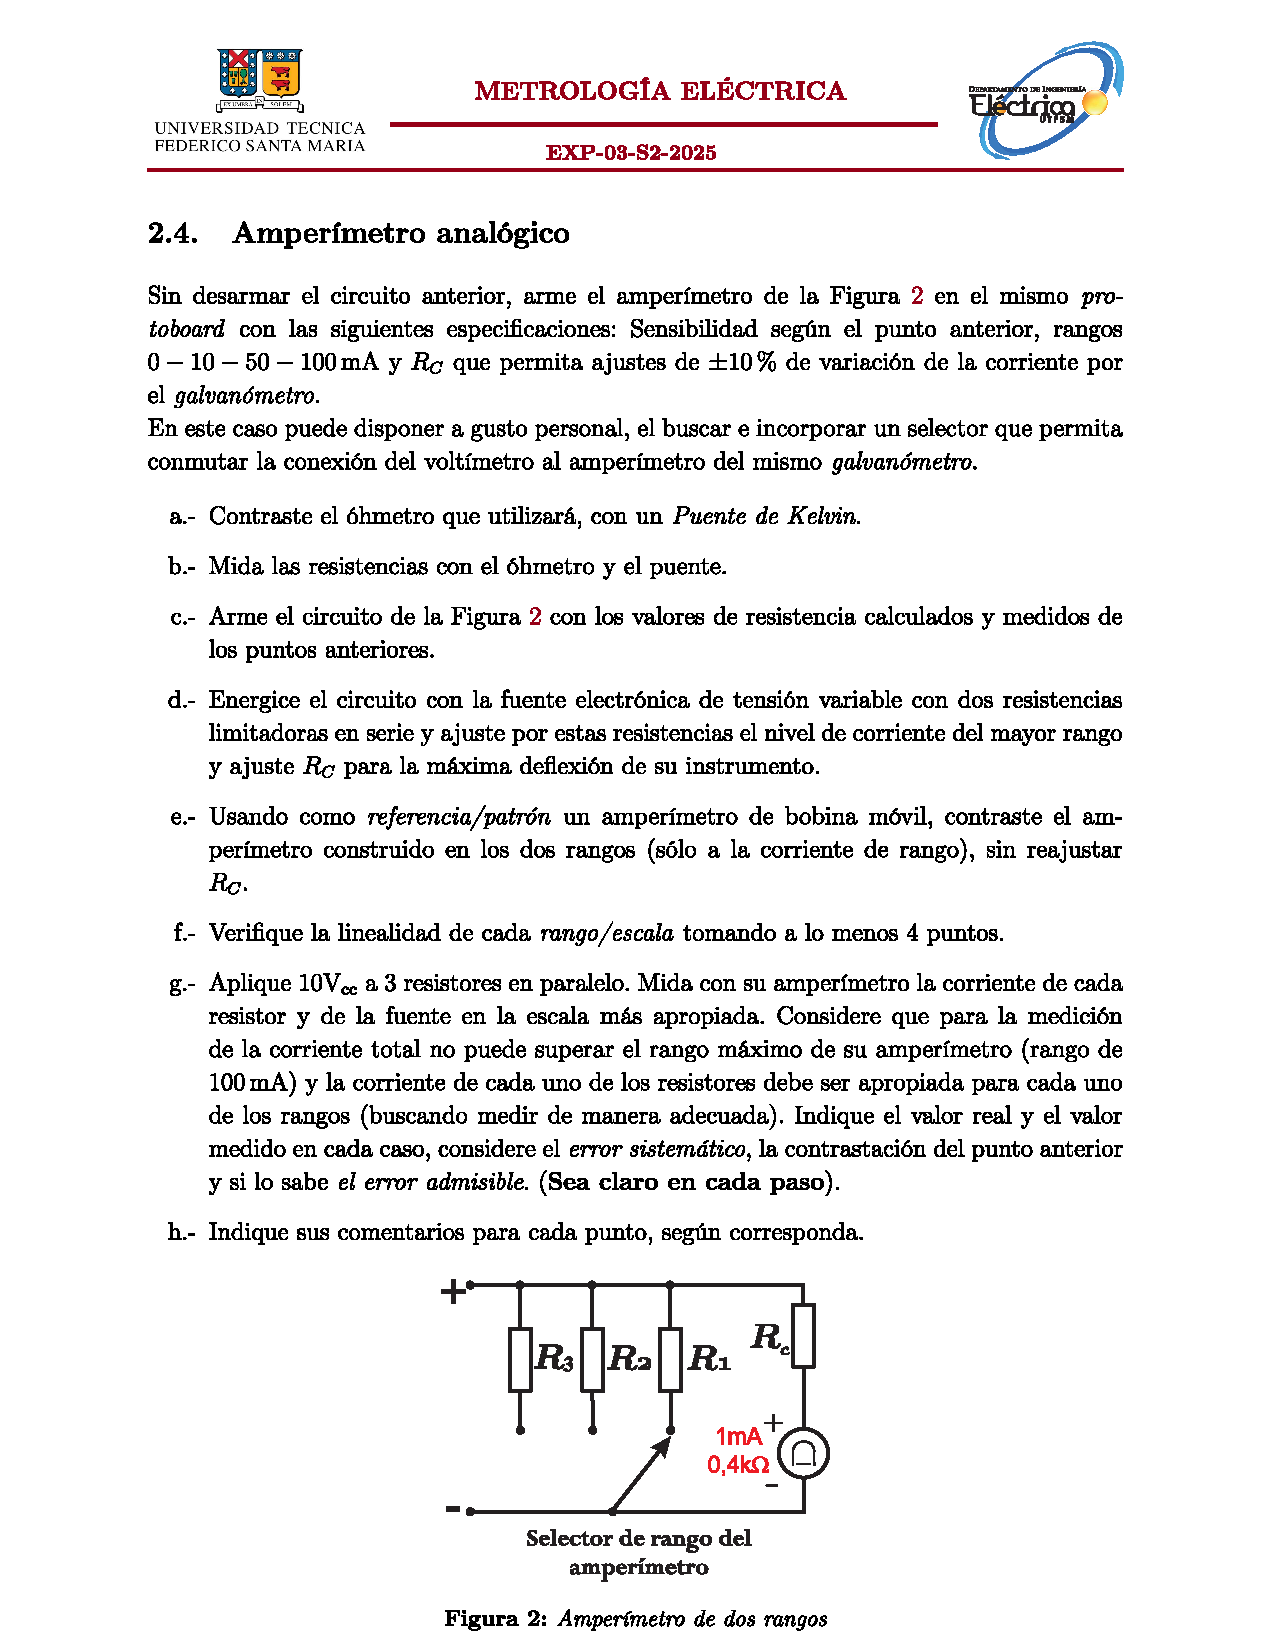
\includegraphics[    angle=0,
    trim=50mm 12mm 50mm 216mm, % izq abajo der arriba
    clip,
    width=\linewidth]{recursos/ammeter.pdf}
  \caption{Esquema circuital del amperímetro de rango variable.}
  \label{fig:ammeter}
\end{figure}

La resistencia de calibración se calcula a partir de la relación entre la corriente que pasa por el galvanómetro $I_g$ y la corriente total $I$ medida por el amperímetro. Usando el cálculo de las resistencias shunt y la ecuación de la corriente a través del galvanómetro, se determina $R_c$ como la resistencia que satisface la relación de corrientes que se desprende del análisis circuital del amperímetro descrito en la figura \ref{fig:ammeter}, tal que:

\[
R_sI - R_sI_g=(R_c+R_g)I_g \Leftrightarrow I = I_g\frac{R_c+R_g+Rs}{R_s}
\]

Donde $I$ corresponde a la corriente máxima a medir en el rango en cuestión, e $I_g$ sea la corriente máxima que es capaz de soportar el galvanómetro.

\subsubsection{Protecciones del Instrumento}
Para proteger al galvanómetro de sobrecorrientes, se incorporan diodos en antiparalelo. Los diodos tienen la característica de que no consumen corriente cuando están en su estado normal, pero cuando la corriente excede un valor umbral (típicamente $0.7 \ [V]/R_g$), los diodos se comportan como cortocircuitos, desviando la corriente y evitando daños en el instrumento.

\subsubsection{Circuito de Contrastación del Amperímetro}
Para verificar el correcto funcionamiento de los rangos diseñados, se implementa un circuito de contrastación. A diferencia de un ajuste tradicional con resistencias variables, en esta experiencia se empleó una resistencia limitadora $R_{lim}$ fija y conocida para cada rango, conectada en serie con el amperímetro bajo prueba y un amperímetro patrón. La variación de corriente, necesaria para tomar múltiples puntos y verificar la linealidad, se logró ajustando la tensión de alimentación de una fuente DC variable desde 10 V hacia abajo. El esquema de este circuito se presenta y diseña en detalle en la sección de trabajo previo.
\subsubsection{Circuito de Validación del Amperímetro}
Con el fin de estudiar el error sistemático del instrumento, se diseñó un circuito de validación compuesto por tres resistencias en paralelo alimentadas por una fuente de 10 V DC. Los valores seleccionados ($R_1 = 1\,\text{k}\Omega$, $R_2 = 330\,\Omega$ y $R_3 = 220\,\Omega$) garantizan que las corrientes de rama sean medibles en los rangos menores (aproximadamente 10 mA, 30 mA y 45 mA respectivamente), mientras que la corriente total del nodo principal no supera el rango máximo de 100 mA del instrumento construido. El esquema y cálculo de este arreglo se detalla en el trabajo previo.
\subsubsection{Puente de Kelvin}
Cuando las resistencias $N$ y $n$ se ajustan de modo que la corriente que fluye por el galvanómetro $G$ tiende a cero, la resistencia desconocida $X$ e expresa mediante la ecuación~\eqref{eq:6.1} de la siguiente forma:

\begin{equation}
X = \frac{N}{M} \times S + \frac{m \times \ell}{m + n + \ell} 
\times \left( \frac{N}{M} - \frac{n}{m} \right)
\label{eq:6.1}
\end{equation}

donde $\ell$ es la resistencia de los conductores de conexión desde el terminal $P_s$ de $S$ hasta el terminal $P_x$ de $X$.

\begin{figure}[H]
    \centering
    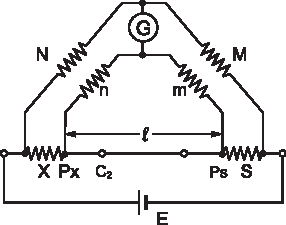
\includegraphics[width=0.5\textwidth]{recursos/kelvin.pdf}
    \caption{Diagrama teórico del circuito del Puente de Kelvin.}
    \label{fig:puente_kelvin}
\end{figure}


El puente de Kelvin está diseñado de modo que las resistencias fijas y las resistencias deslizantes mantienen la siguiente relación:

\[
N = n \quad \text{y} \quad M = m
\]

Por lo tanto:

\[
\frac{N}{M} - \frac{n}{m} = 0
\]

A partir de la ecuación~\eqref{eq:6.1}, se obtiene:

\begin{equation}
X = \frac{N}{M} \times S
\label{eq:6.2}
\end{equation}

Entonces la resistencia baja $X$ puede medirse con gran precisión sin verse afectada por la resistencia de conexión $\ell$.

